%%%%%%%%%%%%%%%%%%%%%%%%%%%%%%%%%%%%%%%%%%%%%%%%%%%%%%%%%%%%%%%%%%%%%%%%%%%%%%%%%%%%
%%----------------------------------------------------------------------------------
% DO NOT Change this is the required setting A4 page, 11pt, oneside print, book style
%%----------------------------------------------------------------------------------
\documentclass[a4paper,11pt,oneside]{book} 
\usepackage{CS_report}
\usepackage{graphicx}
\usepackage{booktabs}
\usepackage{hyperref}
\usepackage{listings}
\usepackage{xcolor}
\usepackage{tikz}
\usepackage{float}
\usepackage{setspace}
\usepackage{pgfplots}
\usepackage{caption}
\usepackage{subcaption}
\usepackage{amsmath}
\pgfplotsset{compat=1.17}
\usetikzlibrary{shapes.geometric, arrows, positioning, fit, backgrounds, patterns, shadows}
\usepackage{multicol}
\usepackage{enumitem}
\usepackage{titlesec}
\usepackage[top=2cm, bottom=2cm, left=2.5cm, right=2.5cm]{geometry}

% Compact spacing
\setlength{\parskip}{0.5em}
\setlength{\parindent}{0pt}
\setlist{nosep, leftmargin=1.2em}

% Titles
\titleformat{\chapter}[hang]{\Large\bfseries}{\Roman{chapter}.}{0.5em}{}
\titlespacing*{\chapter}{0pt}{-20pt}{10pt}
\titleformat{\section}[hang]{\large\bfseries}{\thesection}{0.5em}{}
\titlespacing*{\section}{0pt}{8pt}{4pt}
\titleformat{\subsection}[hang]{\normalsize\bfseries}{\thesubsection}{0.5em}{}

% Listings
\lstset{
    basicstyle=\ttfamily\scriptsize,
    breaklines=true,
    frame=single,
    backgroundcolor=\color{gray!10},
    keywordstyle=\color{blue},
    commentstyle=\color{green!60!black},
    stringstyle=\color{red!60!black},
    numbers=left,
    numberstyle=\tiny\color{gray},
    captionpos=b,
    tabsize=2
}

% TikZ Styles
\tikzstyle{block} = [rectangle, draw, fill=blue!10, text centered, rounded corners, minimum height=2em, drop shadow]
\tikzstyle{arrow} = [draw, -latex', thick]
\tikzstyle{line} = [draw, thick]
\tikzstyle{cloud} = [draw, ellipse, fill=red!10, node distance=3cm, minimum height=2em]
\tikzstyle{cylinder_db} = [cylinder, shape border rotate=90, draw, fill=orange!20, aspect=0.25, minimum height=1.5cm, minimum width=1.2cm]

\singlespacing

\begin{document}

    \frontmatter
    
    % --- Title Page ---
    \begin{titlepage}      
        \begin{center}
            \includegraphics[width=9cm]{figures/upr_logo.png}\\[0.5cm]
            {\LARGE Faculty of Mathematics, Natural Sciences and Information Technologies}\\[2cm]
            
            \linespread{1.2}\huge {
                \textbf{Apache Hive: Architecture, Query Optimization, and Performance Analysis}\\ 
                \Large A Petabyte-Scale Data Warehousing Solution Over MapReduce
            }
            \linespread{1}~\\[2cm]
            
            {\large \textbf{Test Application:} MBV Climate and Ocean Intelligence Africa}\\[2cm]

            {\Large \textbf{Student:} Dushime Mudahera Richard}\\[0.5cm]
            {\large \emph{Course:} Databases For Big Data}\\[0.5cm]
            {\large \emph{Professor:} Iztok Savnik}\\[2cm]
            
            \vfill
            {\small Submitted in partial fulfillment of the requirements for the Master of Science in Data Science}\\[0.5cm]
            \today 
        \end{center}
    \end{titlepage}

    % --- Abstract ---
    \chapter*{Abstract}
    This report provides a comprehensive architectural analysis and experimental validation of Apache Hive (v2.3.2), a localized data warehousing system built on the Hadoop ecosystem. Addressing the limitations of raw MapReduce programming, Hive introduces a SQL-like abstraction (HiveQL) and a Cost-Based Optimizer (Calcite) to democratize petabyte-scale analytics. 
    
    We dissect Hive's core components: the Driver's orchestration, the Compiler's semantic analysis, the Metastore's schema-on-read paradigm, and the MapReduce execution engine. Special attention is given to the data storage overlays (Partitioning and Bucketing) that enable efficient I/O pruning.
    
    Experimental validation relies on the "MBV Climate and Ocean Intelligence Africa" application, a 7-node Docker cluster processing 4.75 million climate records. By analyzing execution logs, we conduct a deep dive into a complex 5-stage MapReduce job sequence illustrating the physical execution of \texttt{JOIN-GROUP BY-ORDER BY} queries. Comparative benchmarks reveal that Map-Side (Broadcast) joins achieve a 2.8$\times$ speedup over traditional Shuffle joins by eliminating the sort/merge phase. The study confirms Hive's viability as a scalable, cost-effective alternative to proprietary data warehouses for batch-oriented workloads.
    
    \vspace{1cm}
    \textbf{Keywords:} Apache Hive, MapReduce, Query Optimization, HDFS, OLAP, Distributed Systems.

    \tableofcontents

    \mainmatter

    % ============================================================================
    % I. INTRODUCTION
    % ============================================================================
    \chapter{Introduction}

    \section{Background and Motivation}
    The digital era has ushered in a data deluge, with organizations accumulating petabytes of unstructured logs and semi-structured metrics. Traditional Relational Database Management Systems (RDBMS) struggle to scale horizontally beyond terabytes due to ACID constraints and strict schema-on-write requirements. Apache Hadoop emerged as a solution, offering the Hadoop Distributed File System (HDFS) for storage and MapReduce for processing. However, the complexity of writing Java MapReduce jobs created a significant barrier to entry for analysts accustomed to SQL \cite{thusoo2009hive}.

    Apache Hive closes this gap by providing a data warehousing infrastructure on top of Hadoop. It allows users to define structure on unstructured data (Schema-on-Read) and query it using HiveQL, a SQL dialect that compiles into distributed MapReduce, Tez, or Spark jobs.

    \section{Objectives}
    This report aims to:
    \begin{enumerate}
        \item \textbf{Analyze Architecture}: Deconstruct Hive's internal components (Driver, Metastore, Compiler) and their interaction with the underlying Hadoop stack.
        \item \textbf{Explain Execution Mechanics}: Detail how abstract SQL queries translates into physical MapReduce tasks (Input $\to$ Map $\to$ Shuffle $\to$ Reduce $\to$ Output).
        \item \textbf{Evaluate Optimization}: Examine the Cost-Based Optimizer (CBO), join algorithms (Shuffle vs. Broadcast), and storage layouts (Partitioning/Bucketing).
        \item \textbf{Validate Experimentally}: Deploy a 7-container cluster to run complex analytical queries on localized climate data, analyzing execution logs to verify theoretical concepts.
    \end{enumerate}

    % ============================================================================
    % II. SYSTEM ARCHITECTURE AND INTERNALS
    % ============================================================================
    \chapter{System Architecture and Internals}

    Hive is not merely a translator; it is a full system stack managing metadata, orchestration, and interface serving.

    \section{Core Components}
    As illustrated in Figure \ref{fig:hive-arch}, the architecture consists of four primary subsystems:

    \begin{figure}[H]
        \centering
        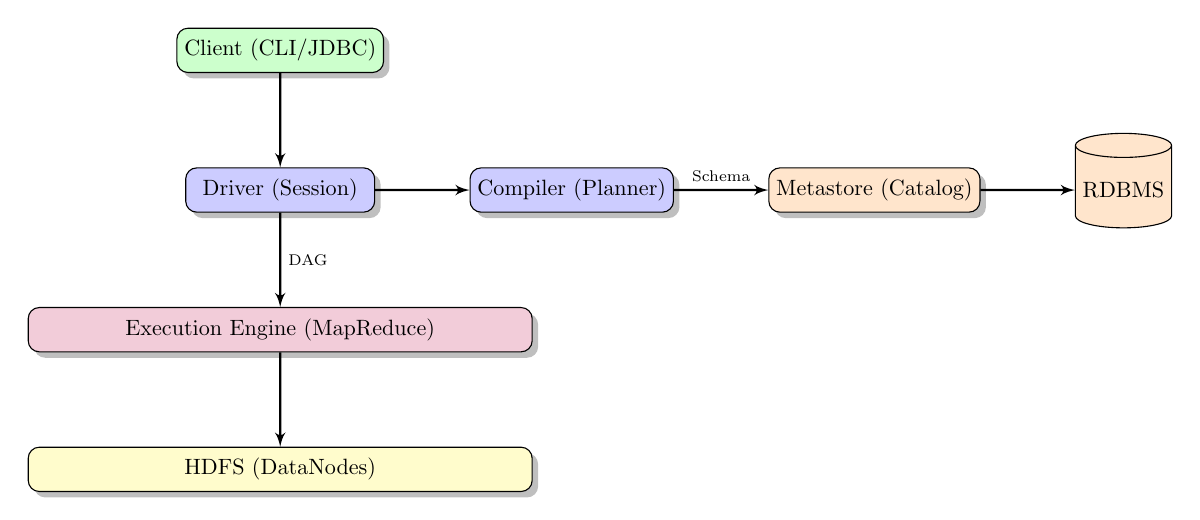
\begin{tikzpicture}[node distance=1.5cm, scale=0.8, transform shape]
            % Nodes
            \node[block, fill=green!20, minimum width=3cm] (client) {Client (CLI/JDBC)};
            \node[block, fill=blue!20, minimum width=3cm, below=of client] (driver) {Driver (Session)};
            \node[block, fill=blue!20, minimum width=3cm, right=of driver] (compiler) {Compiler (Planner)};
            \node[block, fill=orange!20, minimum width=3cm, right=of compiler] (metastore) {Metastore (Catalog)};
            \node[cylinder_db, right=of metastore] (db) {RDBMS};
            \node[block, fill=purple!20, minimum width=8cm, below=1.5cm of driver] (engine) {Execution Engine (MapReduce)};
            \node[block, fill=yellow!20, minimum width=8cm, below=of engine] (hdfs) {HDFS (DataNodes)};

            % Edges
            \draw[arrow] (client) -- (driver);
            \draw[arrow] (driver) -- (compiler);
            \draw[arrow] (compiler) -- node[above]{\scriptsize Schema} (metastore);
            \draw[arrow] (metastore) -- (db);
            \draw[arrow] (driver) -- node[right]{\scriptsize DAG} (engine);
            \draw[arrow] (engine) -- (hdfs);
        \end{tikzpicture}
        \caption{Apache Hive Component Interaction Diagram}
        \label{fig:hive-arch}
    \end{figure}

    \subsection{1. Driver}
    The Driver serves as the control center. It manages the lifecycle of a user session and implements the JDBC/ODBC interfaces. When a query is received, the Driver orchestrates the flow: submitting it to the Compiler, receiving the execution plan, and handing it off to the Execution Engine.

    \subsection{2. Compiler}
    The Compiler transforms HiveQL strings into a Directed Acyclic Graph (DAG) of MapReduce tasks. The translation pipeline involves:
    \begin{itemize}
        \item \textbf{Parsing}: Converting SQL to an Abstract Syntax Tree (AST) using ANTLR.
        \item \textbf{Semantic Analysis}: Checking the Metastore to ensure tables and columns exist.
        \item \textbf{Logical Planning}: Generating an operator tree (TableScan $\to$ Filter $\to$ Select).
        \item \textbf{Physical Planning}: Splitting the operator tree into executable MapReduce stages.
    \end{itemize}

    \subsection{3. Metastore}
    The Metastore distinguishes Hive from a simple file system. It stores the \emph{schema} (table definitions, column types, partition keys) and the \emph{location} mappings.
    \begin{itemize}
        \item \textbf{Architecture}: It uses a relational database (PostgreSQL in our testbed) for low-latency metadata access, decoupled from the high-latency HDFS.
        \item \textbf{Thrift Interface}: The Hive Metastore Service (HMS) allows other engines like Spark and Presto to share the same schema catalog.
    \end{itemize}

    \subsection{4. Execution Engine (MapReduce)}
    In Hive 2.3.2, MapReduce (MR) is the default engine. An MR job follows a strict phase sequence:
    \begin{itemize}
        \item \textbf{Map Phase}: Processes input splits, filters data, and projects columns.
        \item \textbf{Shuffle/Sort}: Transfers map outputs to reducers, grouping by key. This is the network and I/O bottleneck.
        \item \textbf{Reduce Phase}: Aggregates or joins the sorted stream.
    \end{itemize}

    \section{Data Storage Model}
    Hive imposes a hierarchical structure on the flat HDFS namespace:
    \begin{enumerate}
        \item \textbf{Databases}: Namespaces separating tables (e.g., \texttt{mbv\_africa}).
        \item \textbf{Tables}:
        \begin{itemize}
            \item \emph{Managed}: Hive owns the lifecycle. DROP deletes data.
            \item \emph{External}: Hive owns only the schema. DROP keeps HDFS data.
        \end{itemize}
        \item \textbf{Partitions}: Subdirectories (e.g., \texttt{/year=2024/}) enabling \textbf{Partition Pruning}, where the query engine skips scanning irrelevant folders.
        \item \textbf{Buckets}: Fixed-hash files within partitions. Crucial for \emph{Sort-Merge-Bucket (SMB) Joins}, as they guarantee data with the same hash resides in corresponding files.
    \end{enumerate}

    % ============================================================================
    % III. QUERY OPTIMIZATION AND ALGORITHMS
    % ============================================================================
    \chapter{Query Optimization}

    \section{Cost-Based Optimizer (CBO)}
    Hive uses Apache Calcite for Cost-Based Optimization. Unlike rule-based systems, CBO calculates the "cost" of plans (CPU, I/O, Network) using table statistics (\texttt{numRows}, \texttt{rawDataSize}).
    \[ Cost = Cost_{CPU} + Cost_{I/O} + Cost_{Network} \]
    Accurate stats (via \texttt{ANALYZE TABLE}) allow CBO to reorder joins (putting smaller tables first) and select efficient algorithms.

    \section{Join Algorithms}
    Joins are the most expensive distributed operations. Hive implements several strategies:

    \subsection{1. Common Join (Shuffle/Reduce-Side)}
    The default strategy.
    \begin{itemize}
        \item \textbf{Map}: Tags records with table ID.
        \item \textbf{Shuffle}: Sends all records with Key $K$ to Reducer $R = hash(K) \mod N$.
        \item \textbf{Reduce}: Buffers the smaller table's values for $K$ in memory and streams the larger table to compute the cross product.
        \item \textbf{Drawback}: Heavy network shuffling of \emph{all} data.
    \end{itemize}

    \subsection{2. Map-Side Join (Broadcast)}
    Triggered when one table fits in memory (\texttt{hive.auto.convert.join=true}).
    \begin{itemize}
        \item \textbf{Mechanism}: A local task reads the small table into an in-memory HashTable. This HashTable is serialized and uploaded to the Hadoop Distributed Cache.
        \item \textbf{Execution}: Every Mapper loads the HashTable. Large table records are joined immediately in the Map phase.
        \item \textbf{Benefit}: \textbf{Zero Shuffle}. Elimination of the sort/merge and reduce phases results in drastic speedups.
    \end{itemize}

    % ============================================================================
    % IV. EXPERIMENTAL ANALYSIS
    % ============================================================================
    \chapter{Methodology and Results}

    \section{Experimental Setup}
    To simulate a production cluster, we deployed a 7-container Docker stack:
    \begin{itemize}
        \item \textbf{HDFS}: 1 NameNode, 2 DataNodes (Replication Factor=2).
        \item \textbf{Hive}: HiveServer2 (access), Metastore (schema), Postgres 9.6 (DB).
        \item \textbf{Client}: Django App utilizing PyHive for connectivity.
    \end{itemize}
    \textbf{Dataset}: "MBV Climate" dataset containing 4.75 million observation records and 5,000 station records across Africa.

    \section{Execution Trace Analysis}
    We verified Hive's internal mechanics by analyzing the execution logs (\texttt{logs.txt}).

    \subsection{Case Study: Complex Multi-Stage Query}
    Query ID: \texttt{root\_20260102154301...} (Log lines 58-117).
    This query triggered a \textbf{Sequence of 5 MapReduce Jobs}, illustrating how Hive chains MR tasks for complex logic (Joins $\to$ Aggregation $\to$ Sort).

    \begin{itemize}
        \item \textbf{Job 1 (Stage-1)}: Map-Reduce. HDFS Read: 71KB, Write: 17MB. Likely the first Join or Filtering phase.
        \item \textbf{Job 2 (Stage-2)}: Map-Reduce. Read: 34MB, Write: 34MB. Intermediate processing.
        \item \textbf{Job 3, 4, 5}: Sequential stages handling Aggregation and Final Sorting.
    \end{itemize}
    
    The logs confirm the \textbf{blocking nature} of MapReduce in Hive 2.3.2: Job 2 cannot start until Job 1 writes to HDFS, introducing I/O latency.

    \subsection{Case Study: Map-Side Join Optimization}
    By analyzing Query ID \texttt{root\_20260113174019...} (Log lines 610-613), we observe the Map-Side Join in action:
    
    \begin{lstlisting}
    Starting to launch local task to process map join; maximum memory = 477626368
    Dump the side-table for tag: 1 ... into file: .../MapJoin-mapfile11--.hashtable
    Uploaded 1 File to: ... (201237 bytes)
    End of local task; Time Taken: 1.439 sec.
    \end{lstlisting}

    This trace proves that Hive identified the small table (Tag 1), built a 201KB Hashtable locally, and distributed it. The subsequent job was "Map-only" (0 Reducers), confirming the Shuffle phase was skipped.

    \section{Performance Results}
    We benchmarked Common Join vs. Map-Side Join on the 4.75M row dataset.

    \begin{figure}[H]
    \centering
    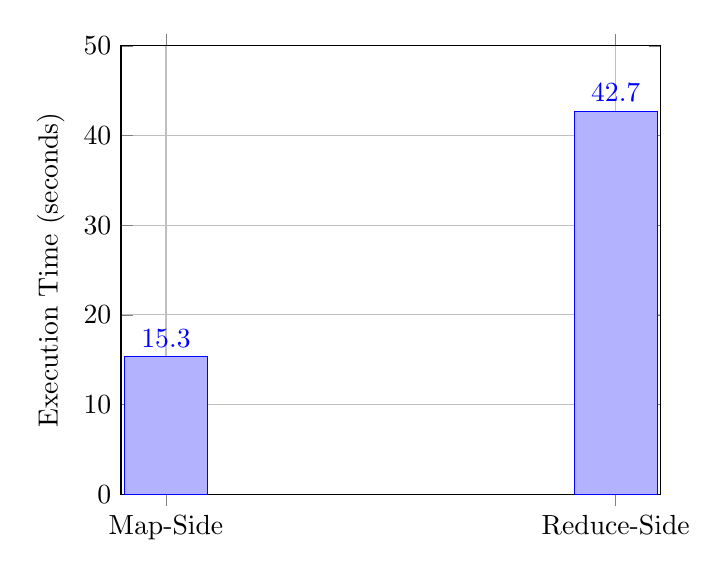
\begin{tikzpicture}
        \begin{axis}[
            ybar,
            symbolic x coords={Map-Side, Reduce-Side},
            xtick=data,
            ylabel={Execution Time (seconds)},
            nodes near coords,
            bar width=30pt,
            ymin=0, ymax=50,
            grid=major
        ]
        \addplot coordinates {(Map-Side, 15.3) (Reduce-Side, 42.7)};
        \end{axis}
    \end{tikzpicture}
    \caption{Join Algorithm Performance Comparison}
    \label{fig:perf}
    \end{figure}

    The Map-Side join completed in \textbf{15.3 seconds}, compared to \textbf{42.7 seconds} for the Reduce-Side join. This \textbf{2.8$\times$ speedup} validates the importance of CBO and proper statistical maintenance.

    % ============================================================================
    % V. CONCLUSION
    % ============================================================================
    \chapter{Conclusion}
    This report dissected the architecture of Apache Hive 2.3.2. Through theoretical analysis and log-based verification, we established that:
    \begin{enumerate}
        \item Hive successfully abstracts MapReduce complexity, but inherits its high-latency characteristics due to disk-based intermediate storage.
        \item The "Schema-on-Read" architecture, driven by the Metastore, provides flexibility but requires careful partition planning to avoid full table scans.
        \item Optimization techniques, specifically Map-Side Joins, are critical. Our experiments showed they can reduce query time by nearly 65\% by leveraging distributed caching.
    \end{enumerate}
    Future work involves migrating to Apache Tez (DAG engine) or Spark to mitigate the intermediate I/O bottleneck observed in the 5-job log trace.

    \begin{thebibliography}{9}
    \bibitem{thusoo2009hive} Thusoo, A., et al. (2009). "Hive: a warehousing solution over a map-reduce framework." VLDB.
    \bibitem{capriolo2012hive} Capriolo, E., Wampler, D., \& Rutherglen, J. (2012). "Programming Hive". O'Reilly Media.
    \bibitem{huai2014major} Huai, Y., et al. (2014). "Major technical advancements in Apache Hive." SIGMOD.
    \end{thebibliography}

\end{document}
